\title{Spezielle Themen der Algorithmik - Blatt 1}
\documentclass[a4paper]{scrartcl}
\usepackage[utf8]{inputenc}
\usepackage[ngerman]{babel}
%\usepackage{fancyhdr}
\usepackage{graphicx}
\setlength{\parindent}{0mm}
%\pagestyle{fancy}




\begin{document}
Das Thema, das ich vorschlagen möchte würde auf der Arbeit aufbauen, die Tricard, Efremov, Zanni, Neyret, Martinez und Lefebvre in "Procedural Phasor Noise" geleistet haben. In diesem Paper führen sie Phasor Noise ein. Hierfür gehen sie von Gabor Noise in folgender Form aus
$$
G(\vec{x}) = \sum_{i=0}^ne^{-\frac{\pi||\vec{x}-\vec{x_i}||^2}{\sigma^2}}\sin(F(\vec{x}-\vec{x}_i)\vec{u})
$$
wobei $\sigma$ Parameter der Gaußschen Glocke ist, $F$ und $\vec{u}$ Frequenz und Richtung der Sinusschwingung sind und $\vec{x}_i$ die Position des $i$-ten Gaborkernels ist. Mittels Phasor-Addition gelingt es ihnen Gabor Noise in folgende Form zu bringen
$$
G(\vec{x}) = I(\vec{x})\sin(F\vec{x}\vec{u}+\varphi(\vec{x}))
$$
wobei $I$ die Hüllkurve von $G$ ist und $\varphi$ die positionsabhängige Phasenverschiebung der Sinusschwingung. Durch entfernen von $I$ erhalten sie eine Phasor-Sinuswelle (Phasor Sinewave). Gegenüber Gabor Noise besitzt diese den Vorteil das sie keine Bereiche besitzt, in denen die Schwingung aufgrund von geringem Kontrast nicht mehr sichtbar ist (vgl. Abbildung \ref{fig:fig}).\\
\\
\begin{figure}[h]
	\centering
	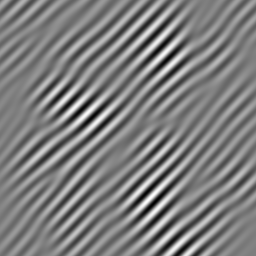
\includegraphics[width=0.3\textwidth]{gaborNoise}
	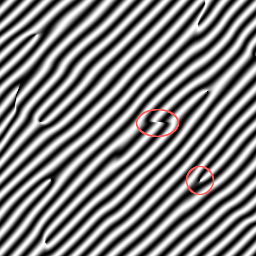
\includegraphics[width=0.3\textwidth]{phasorSineWave}
	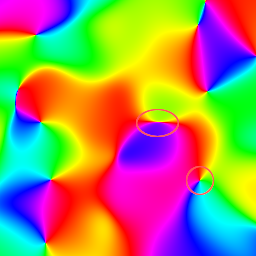
\includegraphics[width=0.3\textwidth]{phasorPhase}
	\caption{Gabor Noise (links), die Entsprechende Phasor Noise Instanz (mitte) und dessen Phasenverschiebung (rechts)}
	\label{fig:fig}
\end{figure}

Dadurch kommen aber andere Artefakte zum Vorschein (vgl. Abbildung \ref{fig:fig}). Tricard et al. stellen bereits fest, dass man diese Artefakte bereits an der Phasenverschiebung ablesen kann.\\
\\
Meine Idee wäre nun die Phasenverschiebung über andere Wege zu generieren um mehr Kontrolle über diese Artefakte zu gewinnen. Vorzugsweise würde ich andere Noise Algorithmen verwenden um die Phasenverschiebung zu generieren und Existenz der unterschiedlichen Artefakttypen und möglicherweise auch deren Position explizit einzustellen.\\
\\
Dies würde folgende Aufgaben nach sich ziehen:
\begin{enumerate}
\item Umsetzung der Generierung in Code
\item Überprüfung wann die Bereich mit geringen Kontrast wieder auftauchen (abhängig von der generierten Phase)\label{p2}
\item Umsetzung für Phasor Noise mit unterschiedlichen Kernels\label{p3}
\end{enumerate}
Für Punkt \ref{p2} haben Tricard et al. bereits einen Großen Teil der Vorarbeit geleistet, indem sie das erneute Auftreten von Bereichen mit geringem Kontrast an Eigenschaften der Phase gebunden haben. Punkt \ref{p3} ist deshalb aufgeführt, da in der Darstellung von Phasor Noise mit mehreren Kernels keine explizite Phasenverschiebung vorkommt.


\bibliography{source}{}
\bibliographystyle{plain}

\end{document}
